\documentclass[11pt]{article}

\usepackage[T1]{fontenc}
\usepackage[utf8]{inputenc}
\usepackage{lmodern}
\usepackage[margin=1in]{geometry}
\usepackage{amsmath,amssymb}
\usepackage{graphicx}
\usepackage{booktabs}
\usepackage{multirow}
\usepackage{array}
\usepackage{caption}
\usepackage{authblk}
\usepackage[authoryear,round]{natbib}
\usepackage{xcolor}
\usepackage[colorlinks=true,linkcolor=blue!50!black,citecolor=blue!50!black,urlcolor=blue!50!black]{hyperref}
\usepackage{lineno}
\usepackage{setspace}

\graphicspath{{../results/figures/}}
\captionsetup{font=small,labelfont=bf}
\setstretch{1.15}
\linenumbers

\title{Prediction of Systemic Lupus Erythematosus from Genotype and Gene-Expression Data: Batch Correction, Leakage-Free Evaluation and the Limits of Multi-Study Pooling}

\author[1]{Aldis Daniel}
\author[1]{R Karthik\thanks{Corresponding author: \href{mailto:bs22b022@smail.iitm.ac.in}{bs22b022@smail.iitm.ac.in}}}
\author[1]{Vasudha Kannan}
\author[1]{Hitesh Kandarpa}
\affil[1]{Indian Institute of Technology Madras, Chennai, India}
\date{}

\begin{document}
\maketitle

\begin{abstract}
\noindent Systemic Lupus Erythematosus (SLE) is a complex autoimmune disease with a strong genetic component and highly variable clinical features, so no single marker predicts disease status well. We compared two complementary data sources for separating SLE cases from healthy controls: (1) genotypes at 30 candidate SNPs in a South Indian case--control cohort ($n = 425$) and (2) bulk expression of 13 genes from the same pathways, pooled from six GEO series ($n = 642$ SLE or control samples from 483 people). Expression data from different studies and platforms were placed on a common log$_2$ scale and corrected with mean-only ComBat. To rule out data leakage, ComBat, gene filtering, scaling and model fitting were all re-estimated inside each training fold, and samples from the same person (repeated time points, cell types or culture conditions) were always kept in the same fold. Performance was summarised with ROC-AUC, precision--recall AUC (PR-AUC) and the Matthews correlation coefficient (MCC) over $10\times5$-fold cross-validation. A dominant SNP encoding with age and sex gave ROC-AUC $0.699 \pm 0.052$, PR-AUC $0.668 \pm 0.063$ and MCC $0.31 \pm 0.10$, a significant gain over additive encoding. The leakage-free expression classifier gave ROC-AUC $0.837 \pm 0.033$ (L1-logistic regression) and $0.915 \pm 0.021$ (XGBoost), almost the same as the leaky protocols. However, a model given only the study label reached ROC-AUC $0.857$ because disease status is strongly confounded with study. Within individual studies, discrimination was lower (sample-weighted ROC-AUC $0.74$ for L1-LR, $0.83$ for XGBoost), and it fell to $0.55$--$0.74$ when whole studies were held out. After batch adjustment, \textit{MTR} remained down-regulated in SLE, matching the top genetic association at the folate-cycle variant \textit{MTRR} A66G. Several effects reported in our earlier, uncorrected analysis (notably the large \textit{TLR2} up-regulation) did not survive adjustment. Our results show that, for pooled multi-study expression data, leakage-free cross-validation is necessary but not sufficient: batch--label confounding has to be measured directly.
\end{abstract}

\noindent\textbf{Keywords:} systemic lupus erythematosus; SNP; gene expression; ComBat; batch effect; data leakage; precision--recall; Matthews correlation coefficient

\section{Introduction}

Systemic Lupus Erythematosus (SLE) is a systemic autoimmune disease characterised by loss of tolerance to self-antigens, auto-antibody production and immune-mediated tissue damage that can affect multiple organs, including the skin, joints, kidneys and central nervous system \citep{tsokos2011}. Accurate classification of SLE matters clinically because it affects the intensity of treatment, organ-specific monitoring and prognosis, yet current criteria are still largely based on clinical and serological features rather than molecular data \citep{aringer2019}. This motivates data-driven machine-learning approaches that use genetic and gene-expression information to refine disease-state prediction and improve patient stratification \citep{figgett2019}.

In this work we take a dual approach and predict disease state from both genotype data and bulk gene-expression data. By analysing the two modalities together we aim to capture both inherited risk signals and the downstream transcriptional changes associated with SLE.

Public expression data make this kind of study possible, but they come with two well-known pitfalls. First, samples pooled from several studies and microarray platforms carry strong batch effects, and simple per-gene standardisation does not remove them \citep{chen2011}. Second, preprocessing steps that are fitted on all samples before cross-validation, or repeated measurements of the same person split across folds, can leak information from the test set into training and inflate performance \citep{kapoor2023}. An earlier version of this analysis used per-gene z-scores across the pooled cohort and reported ROC-AUC, F1 and accuracy on sample-level folds. Here we (i) correct batch effects explicitly with ComBat \citep{johnson2007}, (ii) rebuild the evaluation so that no step sees the test fold and no person appears on both sides of a split, and (iii) report precision--recall AUC and the Matthews correlation coefficient, which are more informative than ROC-AUC and accuracy under class imbalance \citep{saito2015,chicco2020}. We also measure how much of the apparent expression signal is explained by study membership alone.

We tested four hypotheses:
\begin{itemize}
  \item \textbf{H1:} Dominant encoding outperforms additive encoding for SNP-based classification.
  \item \textbf{H2:} Folate-pathway SNPs show the strongest association with SLE.
  \item \textbf{H3:} XGBoost does not substantially outperform logistic regression given the small sample size.
  \item \textbf{H4:} Gene-expression data are more discriminative than SNP data.
\end{itemize}

\section{Datasets}

\subsection{Genotype data}
The SNP genotype data set was taken from \citet{rupasree2016}, a study designed to assess the pathway-level contribution of genetic variation to SLE susceptibility in a South Indian cohort. It comprises 188 SLE patients (178 female, 10 male) and 237 healthy controls (230 female, 7 male), 425 subjects in total. Genotypes at 30 SNP loci were measured using PCR-based methods and are encoded as 0, 1 or 2, the number of copies of the alternate allele. The 30 SNPs span four pathways (folate metabolism, xenobiotic metabolism, Toll-like receptor signalling and STAT4/related immune genes) that have each been linked to autoimmune pathogenesis. Age at sample collection and biological sex are also recorded. There are no duplicated subjects.

\subsection{Gene-expression data}
The gene-expression data set was assembled by manually curating bulk profiles from the NCBI Gene Expression Omnibus \citep{barrett2013}: 1,211 samples from six GEO series (GSE10325, GSE32591, GSE38351, GSE39088, GSE45291, GSE72747) measured on four Affymetrix platforms (GPL96, GPL570, GPL13158, GPL14663). Sample labels (SLE, Healthy Control or Other/Unknown) were derived from the GEO annotations in the \texttt{title} and \texttt{characteristics\_ch1} fields of each GSM entry. Thirteen genes overlapping the SNP pathways were extracted: \textit{MTHFR}, \textit{TYMS}, \textit{MTR}, \textit{MTRR}, \textit{CYP1A1}, \textit{GSTM1}, \textit{GSTT1}, \textit{GSTP1}, \textit{TLR2}, \textit{TLR4}, \textit{TLR7}, \textit{TLR9} and \textit{STAT4}.

While re-checking the annotations we found one labelling error. GSE72747 is a lupus nephritis cohort sampled at three time points (T0, T12, T24), but the curated file labelled the ten T0 samples as Healthy Control. All 30 samples in that series come from patients, so we relabelled the T0 samples as SLE. After this fix the cohort contains 453 SLE, 189 Healthy Control and 569 Other/Unknown samples (Table~\ref{tab:batches}). Other/Unknown samples (mostly other diseases, such as rheumatoid arthritis, and unannotated samples) were used only to estimate batch parameters and were never classified.

\paragraph{Repeated measurements.} Several series profile the same person more than once. GSE10325 contains CD4$^+$ T cells, CD19$^+$ B cells and myeloid cells from each donor. GSE39088 and GSE72747 contain three time points per patient. GSE38351 contains monocytes from the same healthy donors under up to five culture conditions, plus technical replicates. GSE32591 contains tubulointerstitial and glomerular biopsies from the same kidneys. We parsed a subject identifier from each sample title. The 642 SLE and control samples come from 483 distinct people.

\begin{table}[t]
\centering
\caption{Expression batches (GEO series $\times$ platform) after scale harmonisation. Subjects are distinct people inferred from the GEO sample titles.}
\label{tab:batches}
\small
\begin{tabular}{lrrrrr}
\toprule
Batch & Samples & Healthy & SLE & Other/Unknown & Subjects \\
\midrule
GSE10325\_GPL96     & 67  & 28 & 39  & 0   & 25 \\
GSE32591\_GPL14663  & 93  & 29 & 0   & 64  & 58 \\
GSE38351\_GPL570    & 40  & 36 & 0   & 4   & 15 \\
GSE38351\_GPL96     & 34  & 12 & 14  & 8   & 32 \\
GSE39088\_GPL570    & 142 & 64 & 78  & 0   & 90 \\
GSE45291\_GPL13158  & 805 & 20 & 292 & 493 & 805 \\
GSE72747\_GPL570    & 30  & 0  & 30  & 0   & 10 \\
\midrule
Total               & 1211 & 189 & 453 & 569 & \\
\bottomrule
\end{tabular}
\end{table}

\section{Methods}

\subsection{Gene-expression preprocessing}

\paragraph{Batch definition.} Samples measured on different platforms differ technically even within one GEO series, so we defined batch as series $\times$ platform. GSE38351 contains samples on both GPL570 and GPL96, which gives seven batches. Disease is spread very unevenly across them: three batches contain no SLE samples, one contains no healthy controls, and GSE45291 contributes 292 of the 453 SLE samples but only 20 controls.

\paragraph{Scale harmonisation.} Per-batch summaries showed three different scales: raw intensities (GSE10325, GSE38351; medians in the tens to hundreds, maxima in the thousands), log-scale values (GSE32591, GSE45291; medians around 3--10) and values centred near zero (GSE39088, GSE72747; medians near zero with negative values). ComBat assumes batches are on comparable scales, so we harmonised them as follows. Values of $-1.00$ in the raw-intensity series had no within-batch variance and acted as missing-value flags; we set these, and any other non-positive values in those series, to missing. The two raw-intensity series were then transformed as $\log_2(x)$ with no pseudocount. The other four series were left on their original scale. The two centred series cannot be returned to the log$_2$ scale, and their location difference from the other batches is handled by ComBat's mean adjustment. The resulting values are on a harmonised, log$_2$-like scale. These steps act on each sample independently and never use labels.

\paragraph{Gene filtering.} ComBat cannot estimate batch parameters for a gene with zero variance or missing values within a batch. A gene was excluded if, in any batch, its standard deviation was zero or undefined, or if it had any missing value. \textit{TLR9} and \textit{GSTM1} met this condition, leaving 11 genes. No samples were removed.

\paragraph{ComBat batch correction.} Batch effects were corrected with ComBat \citep{johnson2007,leek2012}, an empirical Bayes method that estimates a location (mean) and optionally a scale (variance) adjustment for each gene in each batch and shrinks these toward a prior estimated across genes. Disease state was passed as a covariate (dummy variables for SLE and Other/Unknown, Healthy Control as reference) so that biological group differences are preserved while batch differences are removed. We compared full ComBat (location and scale) with mean-only ComBat (location only). Our implementation follows the parametric model in \texttt{sva} and \texttt{pyComBat} \citep{behdenna2023}, but separates fitting from application so that batch parameters can be estimated on a training fold and applied to a test fold. On the full cohort it reproduced the \texttt{pyComBat} output to within 0.05 log$_2$ units.

For mean-only ComBat the corrected value of gene $g$ in sample $j$ from batch $b$ is
\begin{equation}
y^{*}_{gj} = y_{gj} - \hat{\gamma}^{*}_{gb}\,\hat{\sigma}_g ,
\label{eq:combat}
\end{equation}
where $\hat{\gamma}^{*}_{gb}$ is the shrunken batch location and $\hat{\sigma}_g$ the pooled residual standard deviation. The disease covariate is needed to \emph{estimate} $\hat{\gamma}^{*}_{gb}$, but the correction itself depends only on the sample's batch. A new, unlabelled sample can therefore be corrected using parameters learned on training data alone. Full ComBat also rescales each residual around the covariate-predicted mean, which requires the test sample's label, so it cannot be applied to unlabelled samples without leakage. Together with its instability on 11 genes (Results), this is why we used mean-only ComBat as the primary correction.

\paragraph{Evaluation of batch correction.} On the 11 retained genes we computed, before and after correction: the mean fraction of per-gene variance explained by batch and by disease (one-way ANOVA $R^2$); the batch $R^2$ of the first two principal components of the gene-standardised matrix; silhouette scores for batch and disease labels (Euclidean distance on gene-standardised data); and, in each batch with at least three SLE and three control samples, Cohen's $d$ for SLE versus control, together with its spread and sign concordance across batches. As a sensitivity check that labels did not drive the correction, we also ran mean-only ComBat without the disease covariate.

\subsection{Leakage-free evaluation of the expression classifiers}

Two sources of leakage were present in the earlier analysis. ComBat (and before it, the z-scoring) was fitted once on all samples, including test samples and their labels, and folds were split by sample, so the same person could contribute, for example, a T-cell profile to training and a B-cell profile to testing. To measure the effect of each, we evaluated the same models under four protocols:

\begin{description}
  \item[P0 (original report).] Globally z-scored 13-gene matrix, curated labels, folds split by sample.
  \item[P1.] Mean-only ComBat fitted once on all samples with the disease covariate, folds split by sample.
  \item[P2.] As P1, but all samples from one person are kept in the same fold.
  \item[P3 (leakage-free, primary).] Folds split by person. Within each training fold, gene filtering, ComBat (fitted on the training SLE/control samples plus the unlabelled Other/Unknown samples), feature standardisation and the classifier are estimated. The test fold is corrected with Eq.~\eqref{eq:combat} using the training-fold batch parameters and is never seen during fitting.
\end{description}

Folds were built with stratified group $k$-fold (\texttt{scikit-learn} \citep{pedregosa2011}), grouping on subject and stratifying on batch $\times$ label so that every batch present in a test fold is also present in the training fold. The code asserts that no subject appears in both. Each protocol was run as $10\times5$-fold cross-validation with different random splits.

\paragraph{Confounding checks.} Because disease is unevenly distributed across batches, a classifier can score well by recognising which study a sample came from. We therefore added three analyses to P3: (a) a \emph{batch-only} logistic regression whose only input is the one-hot batch label, which measures how much discrimination is available from study membership alone; (b) \emph{within-batch} ROC-AUC, PR-AUC and MCC, computed from the P3 out-of-fold predictions separately in each batch that contains both classes and combined as a sample-size-weighted mean; and (c) \emph{leave-one-batch-out} (LOBO) validation, in which a whole batch is held out. Because an unseen batch has no ComBat parameters, its gene means were shifted onto the training-set means without using labels.

\subsection{Genotype analysis}

\paragraph{QC and association.} Missingness was calculated for each of the 30 SNPs. Hardy--Weinberg equilibrium (HWE) was tested in controls with an exact test \citep{wigginton2005}. Variants with HWE $p < 0.001$ were flagged as possible genotyping errors but kept, because the deviation could also reflect real biology. For each SNP, a $\chi^2$ test of independence was applied to the $3 \times 2$ genotype-by-outcome table, and $p$-values were corrected across the 30 variants with the Benjamini--Hochberg procedure \citep{bh1995} at FDR $< 0.05$.

\paragraph{Encodings and classification.} Three inheritance models were evaluated for every SNP: additive (dose 0/1/2), dominant (any alternate allele $\rightarrow 1$) and recessive (homozygous alternate only $\rightarrow 1$), each with age and sex as covariates. We fitted L2-penalised logistic regression (LR; $C = 1$) and XGBoost \citep{chen2016xgb} (300 trees, maximum depth 3, learning rate 0.03, subsampling 0.8). Imputation (most frequent genotype) and standardisation were fitted inside each training fold. Because choosing the ``best'' encoding after seeing the cross-validated scores is itself a mild form of selection on the test folds, we also ran a nested version in which the encoding was chosen by an inner 5-fold CV on the training fold only. Genotype data have no repeated subjects and no batches, so stratified $10\times5$-fold CV was used. SHAP values \citep{lundberg2017} from an XGBoost model fitted to all subjects were used descriptively to rank feature contributions.

\subsection{Performance metrics and model comparison}

For every test fold we computed ROC-AUC, PR-AUC (average precision), MCC, F1, balanced accuracy, accuracy and the Brier score, using a probability threshold of 0.5 for the threshold-dependent metrics. PR-AUC is reported because the expression set is imbalanced (70.6\% SLE) and ROC-AUC can look reassuring in that setting \citep{saito2015}. The chance level for PR-AUC equals the prevalence (0.706 for expression, 0.442 for genotypes). MCC is reported because, unlike accuracy and F1, it is high only when a classifier does well on both classes \citep{chicco2020}. We report mean $\pm$ SD over all 50 folds. Two models scored on the same folds were compared with the Nadeau--Bengio corrected resampled $t$-test \citep{nadeau2003}, which accounts for the overlap between training sets.

\subsection{Differential expression}

Following \citet{nygaard2016}, differential expression was tested on the harmonised (uncorrected) data with batch in the model, rather than on the ComBat output, to avoid the over-confidence that comes from correcting with the disease covariate and then testing for disease. For each gene we fitted $\text{expression} \sim \text{SLE} + \text{batch}$ by ordinary least squares on SLE and control samples, with standard errors clustered by subject, and applied BH-FDR correction across the 11 genes.

\subsection{Software and code availability}
All analyses used Python 3.13 with NumPy, pandas, SciPy, statsmodels, scikit-learn 1.9, XGBoost 3.4 and SHAP 0.54. Fixed random seeds are used throughout. The complete pipeline, which regenerates every table and figure from the curated data with one script, is available in the project GitHub repository.

\section{Results}

\subsection{Batch correction}

Before correction, batch explained 91.9\% of the variance of the average gene, and the first principal component separated the centred series from the rest (Fig.~\ref{fig:pca}A, batch $R^2 = 0.97$). Mean-only ComBat reduced the mean batch $R^2$ to 0.131, the PC1 batch $R^2$ to 0.203 and the batch silhouette from 0.404 to 0.056, while the disease silhouette rose from 0.141 to 0.235 (Table~\ref{tab:combat}; Fig.~\ref{fig:pca}B,D). Full ComBat removed more batch variance (mean batch $R^2$ 0.060) but distorted within-dataset effects: it roughly doubled the spread of Cohen's $d$ across datasets (0.55 to 1.14) and produced an implausible SLE-versus-control effect of $d = -13.2$ for \textit{CYP1A1} in GSE45291, which we attribute to unstable scale estimates from only 11 genes. Mean-only correction leaves within-batch differences unchanged by construction, so its Cohen's $d$ values match the uncorrected ones.

The disease covariate itself raises the apparent disease signal. Without it, mean-only ComBat gave a mean disease $R^2$ of 0.192, compared with 0.265 with it. This is the effect described by \citet{nygaard2016}, and it is why we did not run any statistical test on the corrected matrix.

\begin{table}[t]
\centering
\caption{Batch-correction diagnostics on the 11 retained genes. Cohen's $d$ statistics use the four batches with $\geq 3$ SLE and $\geq 3$ control samples.}
\label{tab:combat}
\footnotesize\setlength{\tabcolsep}{4pt}
\begin{tabular}{lcccc}
\toprule
Metric & Before & Full ComBat & Mean-only ComBat & Mean-only, no covariate \\
\midrule
Mean batch $R^2$ (genes)        & 0.919 & 0.060 & 0.131 & 0.095 \\
Mean disease $R^2$ (genes)      & 0.176 & 0.287 & 0.265 & 0.192 \\
PC1 batch $R^2$                 & 0.970 & 0.143 & 0.203 & 0.017 \\
PC2 batch $R^2$                 & 0.938 & 0.014 & 0.043 & 0.117 \\
Silhouette (batch)              & 0.404 & $-0.113$ & 0.056 & 0.040 \\
Silhouette (disease)            & 0.141 & 0.105 & 0.235 & 0.201 \\
SD of Cohen's $d$ across batches & 0.554 & 1.144 & 0.554 & 0.554 \\
\bottomrule
\end{tabular}
\end{table}

\begin{figure}[t]
\centering
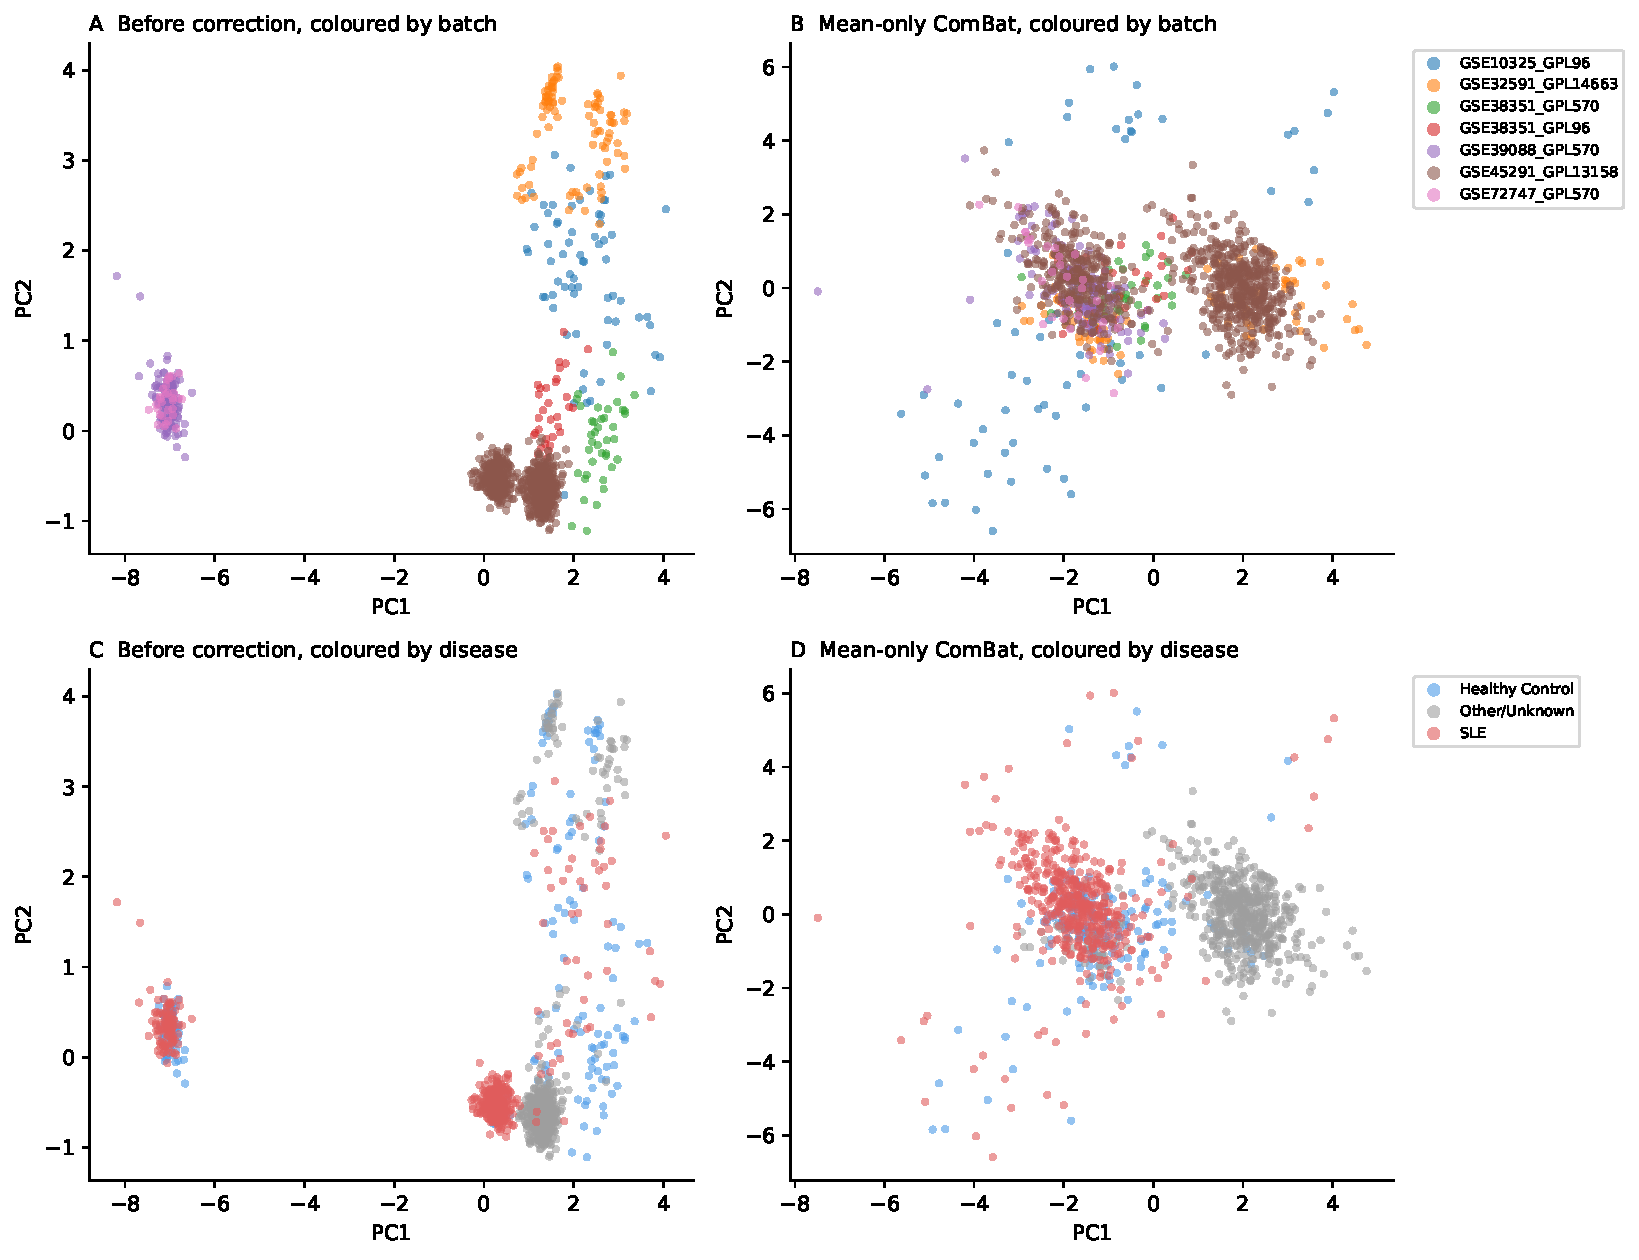
\includegraphics[width=0.92\linewidth]{fig_pca_combat.pdf}
\caption{PCA of the 11-gene expression matrix before and after mean-only ComBat. (A, B) coloured by batch; (C, D) coloured by disease state. Before correction the samples cluster by study and platform; afterwards batches overlap and SLE samples separate from Other/Unknown samples.}
\label{fig:pca}
\end{figure}

\subsection{SNP quality control and association}

Overall missingness was low (mean 0.2\%, maximum 4.7\% for CYP1A1M1). HWE testing in controls flagged four variants at $p < 0.001$, two of them with extreme deviations: \textit{MTRR} A66G ($p = 1.8 \times 10^{-12}$) and \textit{TLR5} rs2072493 ($p = 1.5 \times 10^{-10}$) (Fig.~\ref{fig:snp}A). These may reflect local genotyping difficulty rather than true biological enrichment. Per-SNP $\chi^2$ testing identified four variants at FDR $< 0.05$ (Fig.~\ref{fig:snp}B): \textit{MTRR} A66G ($q = 0.0002$), CYP1A1M2 ($q = 0.014$), \textit{COMT} ($q = 0.032$) and CYP1A1M4 ($q = 0.044$). Seven further SNPs reached nominal significance ($p < 0.05$), including \textit{MTHFR} ($p = 0.034$), \textit{OPN} ($p = 0.032$) and the \textit{TNF}$\alpha$ CCC haplotype ($p = 0.039$). The strongest signal, from the folate-cycle variant \textit{MTRR} A66G, is consistent with H2, although its HWE deviation in controls means it should be confirmed in an independent cohort.

\begin{figure}[t]
\centering
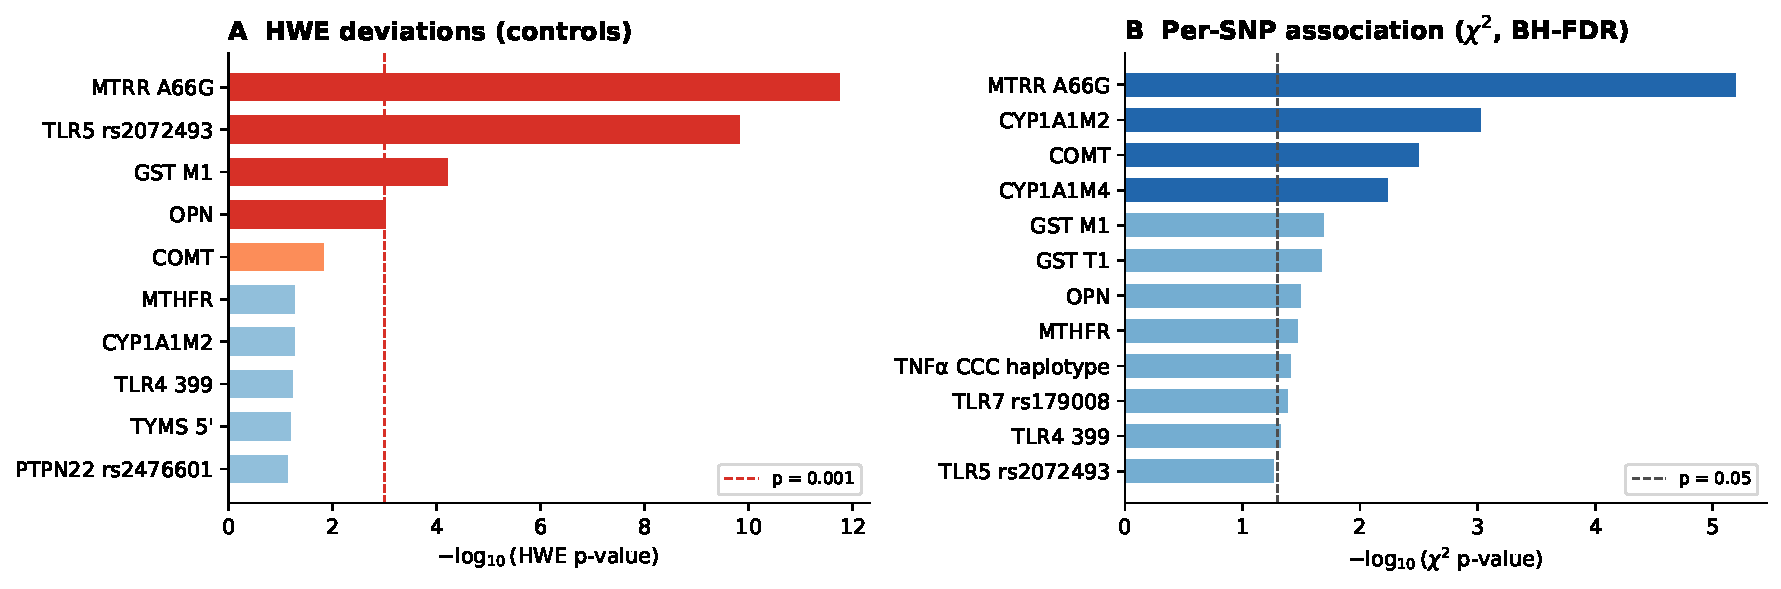
\includegraphics[width=\linewidth]{fig_snp_qc_association.pdf}
\caption{SNP quality control and association. (A) HWE $p$-values in controls ($-\log_{10}$ scale); dashed line at $p = 0.001$. (B) Per-SNP $\chi^2$ association; dark bars indicate BH-FDR $q < 0.05$.}
\label{fig:snp}
\end{figure}

\subsection{SNP classification}

Table~\ref{tab:snp} summarises the repeated cross-validation. Age and sex alone gave ROC-AUC 0.633 and PR-AUC 0.558 (chance 0.442). Adding SNPs under the dominant encoding raised these to 0.699 and 0.668, with MCC rising from 0.18 to 0.31. Dominant encoding beat additive encoding on ROC-AUC (difference 0.044, corrected $p = 0.023$) and PR-AUC (0.046, $p = 0.038$), while the MCC difference (0.097, $p = 0.080$) did not reach significance. Recessive encoding performed worst. When the encoding was chosen inside each training fold, dominant was picked in 48 of 50 folds and performance was essentially unchanged (ROC-AUC 0.696, PR-AUC 0.664), so the H1 result is not an artefact of choosing the encoding on the test folds. XGBoost with additive encoding (ROC-AUC 0.690) did not differ significantly from LR with the same features (ROC-AUC $p = 0.12$; PR-AUC $p = 0.41$), consistent with H3.

SHAP analysis ranked age, \textit{OPN}, \textit{MTRR} A66G, \textit{COMT} and \textit{GST T1} as the top five contributors (Supplementary Fig.~\ref{fig:shap}). Age stands out as a strong non-genetic confounder: controls were older than cases on average (31.4 versus 27.4 years).

\begin{table}[t]
\centering
\caption{SNP classification, $10\times5$-fold stratified CV (mean $\pm$ SD over 50 folds). PR-AUC chance level is 0.442. All models include age and sex.}
\label{tab:snp}
\footnotesize
\begin{tabular}{lcccc}
\toprule
Model & ROC-AUC & PR-AUC & MCC & Balanced acc. \\
\midrule
Age + sex only (LR)          & $0.633 \pm 0.056$ & $0.558 \pm 0.055$ & $0.176 \pm 0.076$ & $0.581 \pm 0.035$ \\
Additive (LR)                & $0.655 \pm 0.046$ & $0.622 \pm 0.057$ & $0.212 \pm 0.100$ & $0.604 \pm 0.050$ \\
Dominant (LR)                & $\mathbf{0.699 \pm 0.052}$ & $\mathbf{0.668 \pm 0.063}$ & $\mathbf{0.309 \pm 0.101}$ & $\mathbf{0.651 \pm 0.050}$ \\
Recessive (LR)               & $0.609 \pm 0.053$ & $0.568 \pm 0.058$ & $0.146 \pm 0.101$ & $0.570 \pm 0.049$ \\
Additive (XGBoost)           & $0.690 \pm 0.054$ & $0.648 \pm 0.066$ & $0.300 \pm 0.105$ & $0.645 \pm 0.051$ \\
Encoding chosen in inner CV (LR) & $0.696 \pm 0.048$ & $0.664 \pm 0.060$ & $0.303 \pm 0.091$ & $0.648 \pm 0.045$ \\
\bottomrule
\end{tabular}
\end{table}

\subsection{Expression classification and data leakage}

Table~\ref{tab:gex} and Fig.~\ref{fig:protocols} show the expression classifiers under the four protocols. P0 reproduces the original report (ROC-AUC $0.807$). Replacing z-scoring with ComBat (P1) improved L1-LR to $0.832$ ROC-AUC and $0.475$ MCC. Moving to subject-grouped folds (P2) and then fitting ComBat inside each fold (P3) changed performance by less than 0.01 on every metric: the leakage-free L1-LR reached ROC-AUC $0.837 \pm 0.033$, PR-AUC $0.920 \pm 0.023$ (chance 0.706) and MCC $0.485 \pm 0.073$. XGBoost was consistently stronger (ROC-AUC $0.915$, PR-AUC $0.963$, MCC $0.640$), and the gap over L1-LR was significant (corrected $p < 10^{-4}$ for ROC-AUC, $p = 0.0003$ for MCC). So, with these data, neither the global ComBat fit nor the repeated subjects inflated the cross-validated estimates noticeably.

\begin{table}[t]
\centering
\caption{Expression classification (SLE vs.\ control, 642 samples, 483 subjects), $10\times5$-fold CV. P0 uses the curated labels of the original report. PR-AUC chance level is 0.706.}
\label{tab:gex}
\footnotesize\setlength{\tabcolsep}{4pt}
\begin{tabular}{llcccc}
\toprule
Protocol & Model & ROC-AUC & PR-AUC & MCC & Balanced acc. \\
\midrule
P0 original (z-score, sample folds) & L1-LR   & $0.807 \pm 0.034$ & $0.899 \pm 0.027$ & $0.335 \pm 0.090$ & $0.641 \pm 0.041$ \\
                                    & XGBoost & $0.908 \pm 0.021$ & $0.954 \pm 0.013$ & $0.602 \pm 0.067$ & $0.790 \pm 0.033$ \\
P1 global ComBat, sample folds      & L1-LR   & $0.832 \pm 0.031$ & $0.918 \pm 0.022$ & $0.475 \pm 0.075$ & $0.713 \pm 0.040$ \\
                                    & XGBoost & $0.913 \pm 0.023$ & $0.961 \pm 0.011$ & $0.625 \pm 0.066$ & $0.799 \pm 0.036$ \\
P2 global ComBat, subject folds     & L1-LR   & $0.837 \pm 0.035$ & $0.920 \pm 0.024$ & $0.477 \pm 0.075$ & $0.713 \pm 0.034$ \\
                                    & XGBoost & $0.913 \pm 0.023$ & $0.962 \pm 0.011$ & $0.628 \pm 0.063$ & $0.802 \pm 0.030$ \\
\midrule
\multirow{3}{*}{P3 leakage-free}    & L1-LR   & $0.837 \pm 0.033$ & $0.920 \pm 0.023$ & $0.485 \pm 0.073$ & $0.718 \pm 0.033$ \\
                                    & XGBoost & $0.915 \pm 0.021$ & $0.963 \pm 0.010$ & $0.640 \pm 0.066$ & $0.811 \pm 0.033$ \\
                                    & Batch label only & $0.857 \pm 0.007$ & $0.910 \pm 0.002$ & $0.519 \pm 0.019$ & $0.672 \pm 0.011$ \\
\bottomrule
\end{tabular}
\end{table}

\begin{figure}[t]
\centering
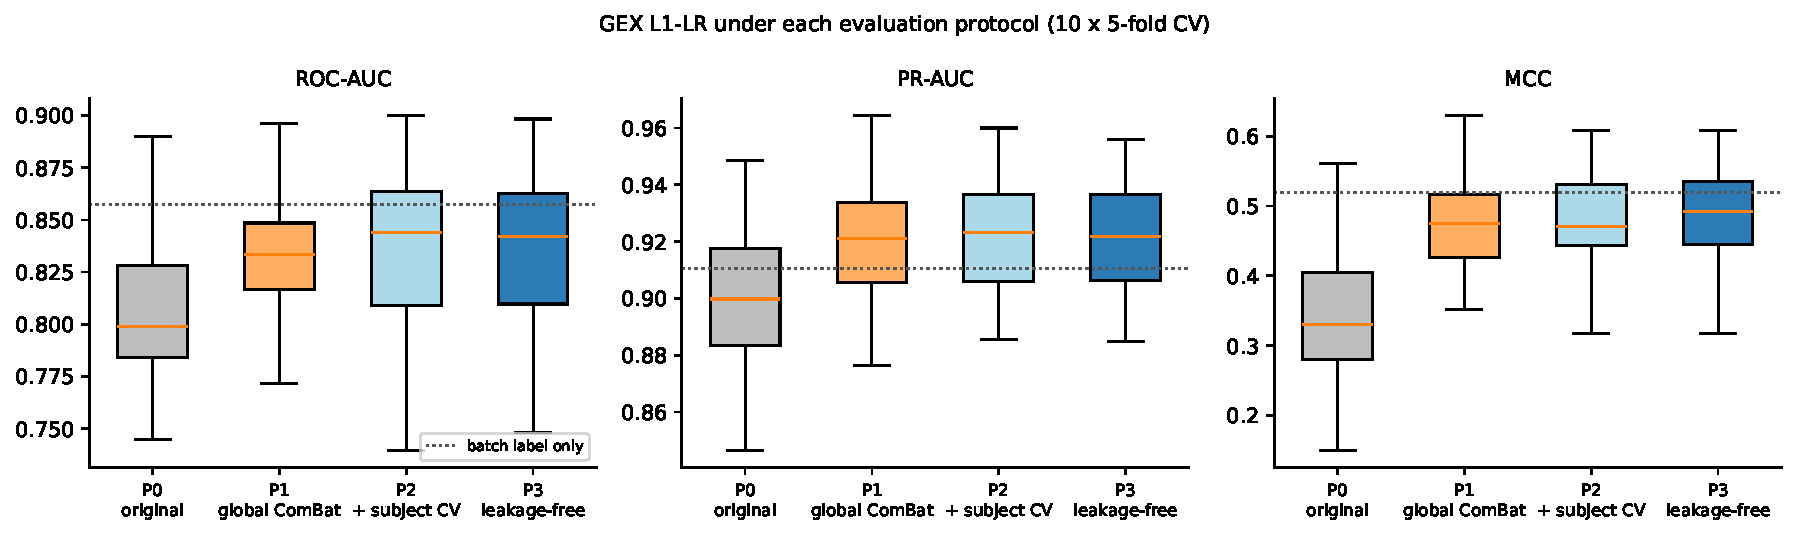
\includegraphics[width=\linewidth]{fig_gex_protocols.pdf}
\caption{Expression L1-LR performance under the four evaluation protocols (50 folds each). The dotted line is the batch-label-only model under the leakage-free protocol.}
\label{fig:protocols}
\end{figure}

\subsection{Study membership explains much of the pooled performance}

The confounding checks show that the pooled estimates in Table~\ref{tab:gex} are not a good guide to how well these genes separate SLE from controls. A logistic regression given only the batch label, with no expression data at all, reached ROC-AUC $0.857$ and MCC $0.519$, higher than the expression L1-LR. This follows directly from Table~\ref{tab:batches}: knowing that a sample comes from GSE45291 or GSE72747 almost guarantees it is SLE, and knowing it comes from GSE32591 or GSE38351\_GPL570 guarantees it is a control.

Within individual batches, where study membership carries no information, discrimination was lower (Table~\ref{tab:within}). The sample-weighted within-batch ROC-AUC was $0.743 \pm 0.006$ for L1-LR and $0.835 \pm 0.006$ for XGBoost (batch-only model: $0.486$). The signal was concentrated in the two whole-blood cohorts, GSE39088 (L1-LR 0.78, XGBoost 0.86) and GSE45291 (0.77, 0.90), and was weak in the sorted-cell and monocyte series GSE10325 and GSE38351 (0.58--0.62). In GSE45291, which is 94\% SLE, L1-LR has a high PR-AUC (0.98) but an MCC near zero (0.01), because at the 0.5 threshold it labels almost every sample SLE. ROC-AUC and PR-AUC alone would have hidden this failure, and MCC exposes it. When whole batches were held out, ROC-AUC fell to 0.55--0.68 for L1-LR and 0.46--0.74 for XGBoost, with MCC between $-0.18$ and $0.15$ (Supplementary Table~\ref{tab:lobo}).

\begin{table}[t]
\centering
\caption{Within-batch discrimination of the leakage-free (P3) out-of-fold predictions, averaged over 10 repeats. Only batches containing both classes are shown.}
\label{tab:within}
\small
\begin{tabular}{lrrcccccc}
\toprule
 & & & \multicolumn{3}{c}{L1-LR} & \multicolumn{3}{c}{XGBoost} \\
\cmidrule(lr){4-6}\cmidrule(lr){7-9}
Batch & $n$ & SLE (\%) & ROC & PR & MCC & ROC & PR & MCC \\
\midrule
GSE10325\_GPL96    & 67  & 58.2 & 0.588 & 0.724 & 0.066 & 0.580 & 0.656 & 0.166 \\
GSE38351\_GPL96    & 26  & 53.8 & 0.576 & 0.651 & 0.150 & 0.621 & 0.607 & 0.247 \\
GSE39088\_GPL570   & 142 & 54.9 & 0.784 & 0.836 & 0.398 & 0.855 & 0.899 & 0.535 \\
GSE45291\_GPL13158 & 312 & 93.6 & 0.771 & 0.981 & 0.009 & 0.898 & 0.991 & 0.475 \\
\midrule
Weighted mean      & 547 &      & 0.743 & 0.896 & 0.124 & 0.835 & 0.908 & 0.442 \\
\bottomrule
\end{tabular}
\end{table}

Figure~\ref{fig:rocpr} compares the out-of-fold ROC and precision--recall curves of both modalities.

\begin{figure}[t]
\centering
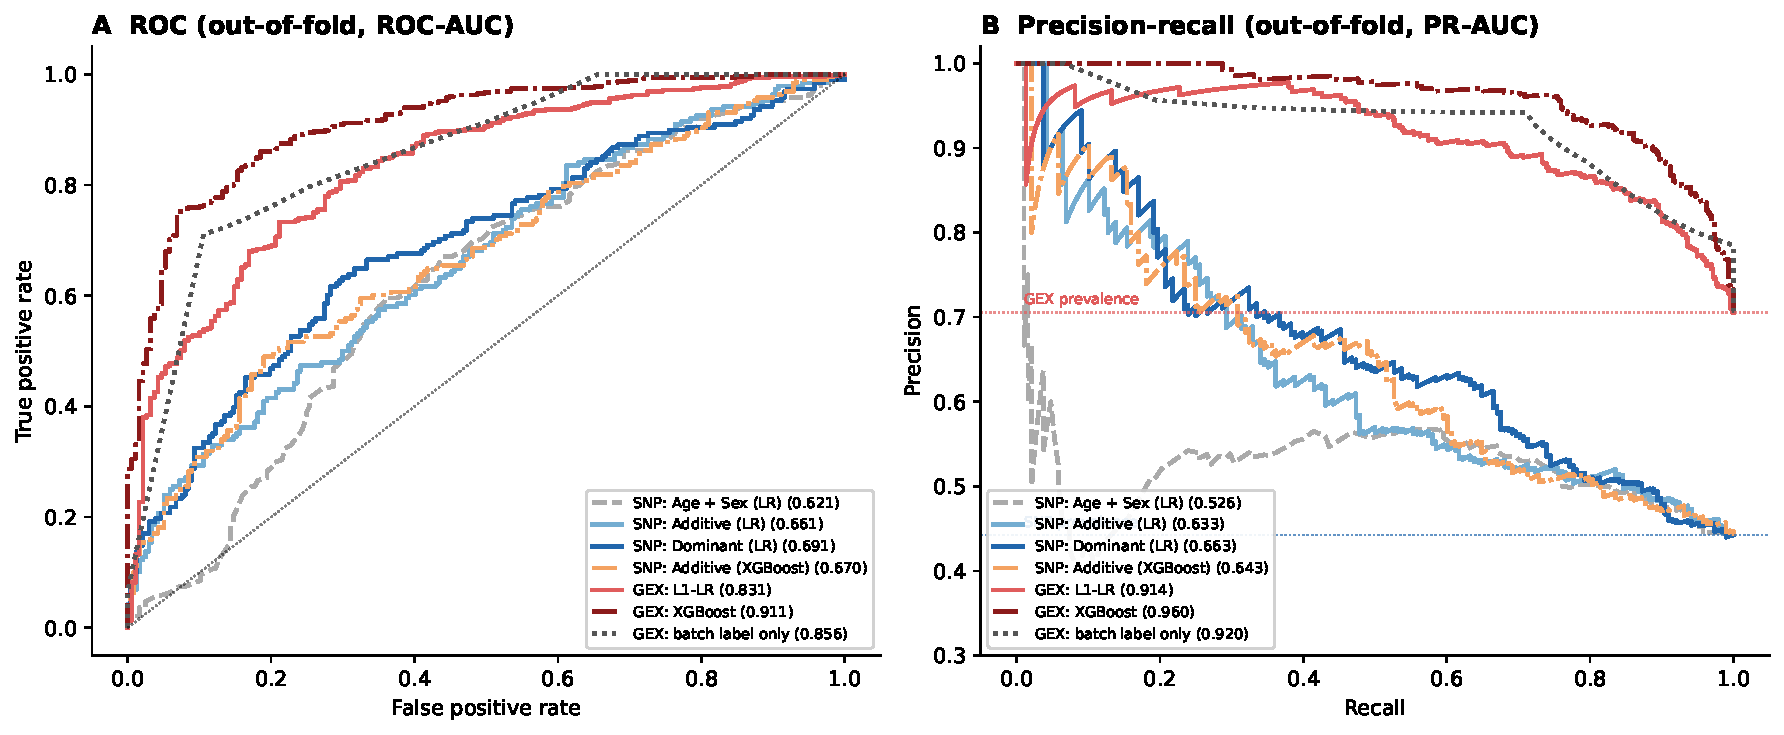
\includegraphics[width=\linewidth]{fig_roc_pr.pdf}
\caption{Out-of-fold ROC (A) and precision--recall (B) curves for the SNP models and the leakage-free (P3) expression models, first CV repeat. Dotted horizontal lines in (B) mark the prevalence (chance PR-AUC) of each data set. The SNP and expression curves come from different cohorts and are not directly comparable.}
\label{fig:rocpr}
\end{figure}

\subsection{Differential expression}

After adjusting for batch, 4 of the 11 genes were differentially expressed at FDR $< 0.05$ (Fig.~\ref{fig:de}; Supplementary Table~\ref{tab:de}): \textit{MTR} ($\log_2$FC $= -0.32$, $q = 6 \times 10^{-5}$), \textit{TYMS} ($+0.34$, $q = 2 \times 10^{-4}$), \textit{STAT4} ($-0.24$, $q = 0.003$) and \textit{GSTP1} ($-0.18$, $q = 0.012$). \textit{TLR2} was nominally up-regulated ($+0.18$, $p = 0.028$, $q = 0.062$). These results differ from our earlier, unadjusted Mann--Whitney analysis on the pooled z-scores, which had reported 9 of 13 genes as significant, a large \textit{TLR2} up-regulation ($\log_2$FC $+2.39$), down-regulation of \textit{MTRR} and up-regulation of \textit{STAT4}. Those effects mostly reflected which studies contributed cases and which contributed controls. Of the earlier findings, only the down-regulation of \textit{MTR} is still supported.

\begin{figure}[t]
\centering
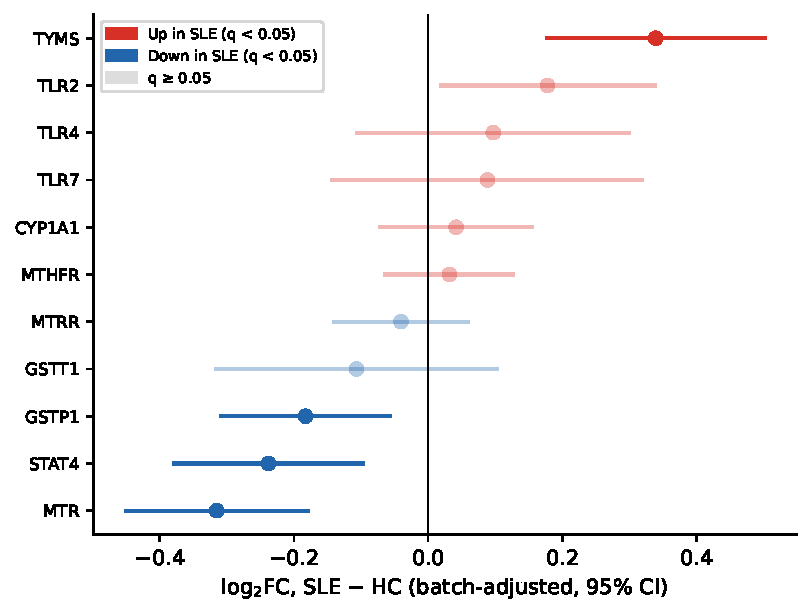
\includegraphics[width=0.62\linewidth]{fig_de_batch_adjusted.pdf}
\caption{Batch-adjusted differential expression (SLE $-$ control) with 95\% confidence intervals (OLS with batch fixed effects, subject-clustered standard errors). Faded points are not significant at BH-FDR $q < 0.05$.}
\label{fig:de}
\end{figure}

\section{Discussion}

\paragraph{Hypotheses.} H1 is supported. Dominant encoding improved ROC-AUC and PR-AUC over additive encoding, the gain survived a corrected paired test, and dominant encoding was also the one chosen inside the training folds. This fits the biology: many autoimmune risk alleles act through haploinsufficiency or gain of function, where a single copy is enough to change pathway flux. H2 is partly supported. \textit{MTRR} A66G was the strongest genetic association, and \textit{MTR} expression was lower in SLE after batch adjustment. Together these point toward reduced methionine-synthase activity, lower \textit{S}-adenosylmethionine availability and altered DNA methylation in SLE. The earlier claim of concordant \textit{MTRR} down-regulation, however, did not survive batch adjustment, and the HWE deviation at \textit{MTRR} A66G calls for replication. H3 is supported for the genotype data, where XGBoost did not significantly outperform logistic regression on 425 subjects. On the larger and more heterogeneous expression data, XGBoost was clearly better, both pooled and within batches. H4 holds only with a caveat. Pooled expression performance (ROC-AUC 0.84--0.92) is well above the genotype models (0.70), but a large part of it comes from study membership. Within studies, L1-LR (0.74) is only modestly above the best SNP model, while XGBoost (0.83) stays clearly ahead. The two modalities were also measured in different people, so this comparison is indirect.

\paragraph{What the leakage analysis does and does not show.} Fitting ComBat inside each fold and keeping each person in a single fold barely changed the cross-validated scores. For this data set, then, the procedural leakage the earlier analysis was exposed to was not the main source of optimism. That is a useful negative result, but it should not be read as reassurance about the pooled numbers. The batch-only baseline shows that when disease labels are unevenly spread across studies, a classifier can reach a high pooled AUC by learning study identity, even when every preprocessing step is fitted only on training data. Mean-only ComBat with a disease covariate removes batch \emph{location} differences while protecting disease differences, but it cannot remove differences in variance, covariance or tissue composition that remain between a blood cohort and a sorted-cell cohort. A flexible model such as XGBoost can still pick these up. The within-batch and leave-one-batch-out results are therefore the more honest estimates of how these 11 genes generalise.

\paragraph{Why PR-AUC and MCC matter here.} The expression set is 71\% SLE, and one batch is 94\% SLE. In that setting a classifier that calls nearly everything SLE still gets a PR-AUC close to 1 and a respectable accuracy and F1. MCC was the only metric that exposed this behaviour (MCC $\approx 0$ for L1-LR in GSE45291), and it also separated the models more clearly than ROC-AUC did (Table~\ref{tab:gex}). We recommend reporting PR-AUC alongside its chance level, together with MCC, for any imbalanced biomedical classifier.

\paragraph{Limitations.} The genotype cohort is ethnically restricted (South Indian), which limits generalisability. The candidate-gene design of both data sets introduces ascertainment bias, and variants outside these pathways are invisible. Only 11 genes survived filtering, which limits ComBat's empirical Bayes shrinkage and is why full ComBat was unstable. Disease is partly confounded with batch: three batches have no SLE samples, one has no controls, and one contributes most SLE samples. In such designs batch adjustment can bias group differences \citep{nygaard2016}, and some of the remaining between-study heterogeneity reflects real cohort, tissue or platform differences rather than technical batch. The two centred series could not be placed on the log$_2$ scale, so cross-platform comparability relies on ComBat's location adjustment. Subject identities were inferred from GEO sample titles. Where a title did not identify the person, each sample was assumed to come from a different individual. Some healthy-control samples in GSE38351 and GSE39088 were stimulated \textit{in vitro} (e.g.\ with interferons), which may not represent resting healthy blood. Finally, lupus nephritis biopsies in GSE32591 were kept under the curated Other/Unknown label and were not used as SLE cases.

\paragraph{Conclusion.} Pathway-level candidate-gene genotyping gives modest SLE discrimination (ROC-AUC $\approx 0.70$, MCC $\approx 0.31$). The same pathway genes measured at the transcript level discriminate better, but when samples are pooled across public studies, much of the apparent advantage comes from study membership rather than disease biology. Leakage-free cross-validation with fold-wise batch correction is necessary, but it is not sufficient. Batch-only baselines, within-study metrics and held-out-study validation should be reported alongside pooled scores. The folate-cycle axis, in particular \textit{MTRR} A66G and reduced \textit{MTR} expression, remains the most consistent signal across both modalities and is a candidate for validation in a cohort where genotype and expression are measured in the same individuals.

\section*{Acknowledgements}
We thank Prof.\ Meiyappan Lakshmanan for the opportunity to develop this work as a course project in BT3041 (Analysis and Interpretation of Biological Data) at IIT Madras, and for feedback that shaped the batch-correction and evaluation analyses.

\section*{Author contributions}
R Karthik led the team, coordinated the work, identified the data sets, contributed to the later stages of analysis and prepared the manuscript. Aldis Daniel carried out the literature survey, helped define the problem and took part in the manual curation of the expression data set. Vasudha Kannan carried out the preprocessing, normalisation and batch correction of the expression data. Hitesh Kandarpa designed and implemented the analysis pipeline. All authors contributed equally in time spent and approved the final manuscript.

\section*{Competing interests}
The authors declare no competing interests.

\bibliographystyle{plainnat}
\bibliography{refs}

\clearpage
\appendix
\renewcommand{\thefigure}{S\arabic{figure}}
\renewcommand{\thetable}{S\arabic{table}}
\setcounter{figure}{0}
\setcounter{table}{0}
\section*{Supplementary material}

\begin{figure}[h]
\centering
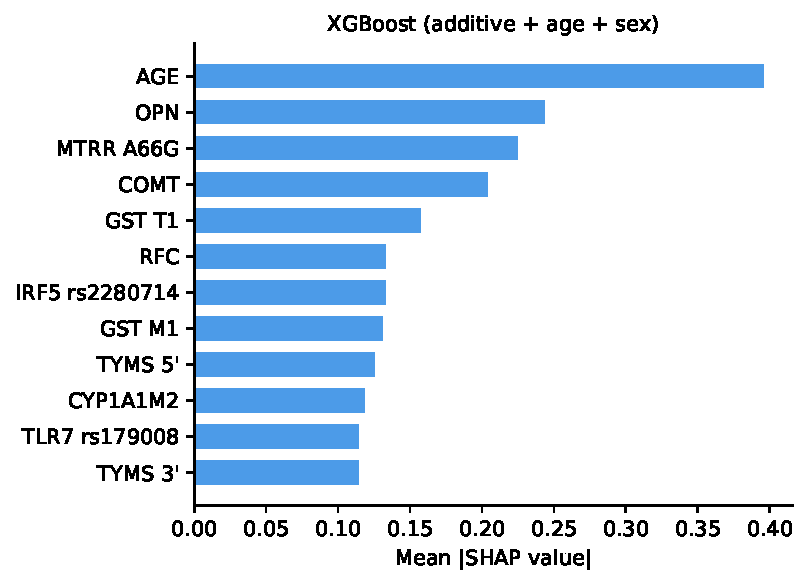
\includegraphics[width=0.6\linewidth]{fig_snp_shap.pdf}
\caption{Mean $|$SHAP$|$ values from XGBoost fitted to all 425 subjects (additive encoding plus age and sex). Descriptive only; not used for model evaluation.}
\label{fig:shap}
\end{figure}

\begin{table}[h]
\centering
\caption{Leave-one-batch-out validation. The held-out batch is shifted onto the training-set gene means without using labels.}
\label{tab:lobo}
\small
\begin{tabular}{lrrcccccc}
\toprule
 & & & \multicolumn{3}{c}{L1-LR} & \multicolumn{3}{c}{XGBoost} \\
\cmidrule(lr){4-6}\cmidrule(lr){7-9}
Held-out batch & $n$ & SLE & ROC & PR & MCC & ROC & PR & MCC \\
\midrule
GSE10325\_GPL96    & 67  & 39  & 0.553 & 0.629 & 0.071 & 0.463 & 0.529 & 0.028 \\
GSE38351\_GPL96    & 26  & 14  & 0.554 & 0.658 & $-0.181$ & 0.482 & 0.531 & $-0.098$ \\
GSE39088\_GPL570   & 142 & 78  & 0.596 & 0.629 & 0.057 & 0.531 & 0.608 & $-0.087$ \\
GSE45291\_GPL13158 & 312 & 292 & 0.684 & 0.973 & 0.141 & 0.741 & 0.977 & 0.153 \\
\bottomrule
\end{tabular}
\end{table}

\begin{table}[h]
\centering
\caption{Batch-adjusted differential expression, SLE vs.\ control (OLS, expression $\sim$ SLE + batch, subject-clustered SE).}
\label{tab:de}
\small
\begin{tabular}{lrrrr}
\toprule
Gene & $\log_2$FC & 95\% CI & $p$ & $q$ (BH) \\
\midrule
\textit{MTR}    & $-0.315$ & $[-0.451, -0.180]$ & $5\times10^{-6}$ & $6\times10^{-5}$ \\
\textit{TYMS}   & $+0.339$ & $[0.177, 0.502]$   & $4\times10^{-5}$ & $2\times10^{-4}$ \\
\textit{STAT4}  & $-0.238$ & $[-0.378, -0.097]$ & 0.0009 & 0.0033 \\
\textit{GSTP1}  & $-0.183$ & $[-0.308, -0.058]$ & 0.0042 & 0.0116 \\
\textit{TLR2}   & $+0.178$ & $[0.019, 0.338]$   & 0.0283 & 0.0623 \\
\textit{GSTT1}  & $-0.107$ & $[-0.315, 0.102]$  & 0.317 & 0.513 \\
\textit{TLR4}   & $+0.097$ & $[-0.105, 0.300]$  & 0.347 & 0.513 \\
\textit{MTRR}   & $-0.040$ & $[-0.140, 0.059]$  & 0.424 & 0.513 \\
\textit{TLR7}   & $+0.089$ & $[-0.142, 0.319]$  & 0.452 & 0.513 \\
\textit{CYP1A1} & $+0.042$ & $[-0.071, 0.154]$  & 0.466 & 0.513 \\
\textit{MTHFR}  & $+0.032$ & $[-0.064, 0.127]$  & 0.514 & 0.514 \\
\bottomrule
\end{tabular}
\end{table}

\end{document}
